\documentclass{article}

%% PAQUETES

% Paquetes generales
\usepackage[margin=2cm, paperwidth=210mm, paperheight=297mm]{geometry}
\usepackage[spanish]{babel}
\usepackage[utf8]{inputenc}
\usepackage{gensymb}

% Paquetes para estilos
\usepackage{textcomp}
\usepackage{setspace}
\usepackage{colortbl}
\usepackage{color}
\usepackage{color}
\usepackage{upquote}
\usepackage{xcolor}
\usepackage{listings}
\usepackage{caption}
\usepackage[T1]{fontenc}
\usepackage[scaled]{beramono}

% Paquetes extras
\usepackage{amssymb}
\usepackage{float}
\usepackage{graphicx}
\usepackage{url}
\usepackage{color}


%% Fin PAQUETES


% Definición de preferencias para la impresión de código fuente.
%% Colores
\definecolor{gray99}{gray}{.99}
\definecolor{gray95}{gray}{.95}
\definecolor{gray75}{gray}{.75}
\definecolor{gray50}{gray}{.50}
\definecolor{gray25}{gray}{.25}
\definecolor{keywords_blue}{rgb}{0.13,0.13,1}
\definecolor{comments_green}{rgb}{0,0.5,0}
\definecolor{strings_red}{rgb}{0.9,0,0}

%% Caja de código
\DeclareCaptionFont{white}{\color{white}}
\DeclareCaptionFont{style_labelfont}{\color{black}\textbf}
\DeclareCaptionFont{style_textfont}{\it\color{black}}
\DeclareCaptionFormat{listing}{\colorbox{gray95}{\parbox{16.78cm}{#1#2#3}}}
\captionsetup[lstlisting]{format=listing,labelfont=style_labelfont,textfont=style_textfont}

\lstset{
	aboveskip = {1.5\baselineskip},
	backgroundcolor = \color{gray99},
	basicstyle = \ttfamily\footnotesize,
	breakatwhitespace = true,   
	breaklines = true,
	captionpos = t,
	columns = fixed,
	commentstyle = \color{comments_green},
	escapeinside = {\%*}{*)}, 
	extendedchars = true,
	frame = lines,
	keywordstyle = \color{keywords_blue}\bfseries,
	language = Oz,                       
	numbers = left,
	numbersep = 5pt,
	numberstyle = \tiny\ttfamily\color{gray50},
	prebreak = \raisebox{0ex}[0ex][0ex]{\ensuremath{\hookleftarrow}},
	rulecolor = \color{gray75},
	showspaces = false,
	showstringspaces = false, 
	showtabs = false,
	stepnumber = 1,
	stringstyle = \color{strings_red},                                    
	tabsize = 2,
	title = \null, % Default value: title=\lstname
	upquote = true,                  
}

%% FIGURAS
\captionsetup[figure]{labelfont=bf,textfont=it}
%% TABLAS
\captionsetup[table]{labelfont=bf,textfont=it}

% COMANDOS

%% Titulo de las cajas de código
\renewcommand{\lstlistingname}{Código}
%% Titulo de las figuras
\renewcommand{\figurename}{Figura}
%% Titulo de las tablas
\renewcommand{\tablename}{Tabla}
%% Referencia a los códigos
\newcommand{\refcode}[1]{\textit{Código \ref{#1}}}
%% Referencia a las imagenes
\newcommand{\refimage}[1]{\textit{Imagen \ref{#1}}}


\begin{document}
\pagenumbering{roman}
\setcounter{page}{5}

% TÍTULO, AUTORES Y FECHA
\begin{titlepage}
	\vspace*{\fill}
	\begin{center}
		\Large 75.06 Organización de Datos \\
		\Huge TP N°1: Catálogo discográfico \\
		\bigskip\huge\textit{Grupo 07} \\
		\bigskip\bigskip\bigskip\bigskip\bigskip\bigskip
		\bigskip\bigskip\bigskip\bigskip\bigskip\bigskip\bigskip
		\medskip\huge\textit{``Documentación de usuario''} \\
		\date{}
	\end{center}
	\vspace*{\fill}
\end{titlepage}
\newpage



% ÍNDICE
\tableofcontents
\newpage
\pagenumbering{arabic}




% INTRODUCCIÓN
\section{Introducción}
	
	El siguiente documento tiene como objetivo proporcionar al usuario toda la información necesaria para la correcta instalación y utilización del software para el armado de un catálogo musical.
	\par
	Este documento va desde los recaudos a tomar previos a la compilación hasta la forma de utilización de la herramienta en si.
\bigskip




% REQUERIMIENTOS DEL SISTEMA
\section{Requerimientos del sistema}

	Antes de instalar y configurar el programa, asegúrese de que su sistema cumple los requisitos mínimos recomendados, los cuales se encuentran especificados a continuación:
	\medskip

\begin{itemize}
\itemsep=5pt \topsep=0pt \partopsep=0pt \parskip=0pt \parsep=0pt

	\item \textit{Sistemas operativos}: GNU/Linux (x86 y x86-64, distribuciones Linux basadas en RPM y DEB);

	\item \textit{Controlador de versions}: GIT (\url{http://git-scm.com/});

	\item \textit{Compilador}: g++ (\url{http://gcc.gnu.org/});

	\item \textit{Herramientas}: Make (\url{http://www.gnu.org/software/make/}).

\end{itemize}
\bigskip




% DESCARGA DEL SOFTWARE
\section{Descarga del software}

	Para obtener la última versión de este software, diríjase a la línea de comandos (terminal) de su sistema operativo e ingrese el siguiente comando:
	\bigskip

	\colorbox{gray95}{{\ttfamily\footnotesize
	\$ git clone \url{git://github.com/federicomrossi/7506-tp-grupo07.git}\\}}
	\bigskip

	Esto descargará los archivos almacenados en el repositorio, ubicándose en la carpeta \textit{código} los archivos fuentes que hacen a la implementación del programa.
\bigskip\medskip




% PASOS PREVIOS A LA UTILIZACION
\section{Pasos previos a la utilización}

	Antes de poder hacer uso de la aplicación es necesario realizar unas pocas tareas previas para la puesta a punto de la misma. Las mismas serán detalladas en lo que sigue de esta sección.
	\bigskip



% PASOS PREVIOS A LA UTILIZACION - Configuracion del entorno
\subsection{Configuración del entorno}

	Previo a la compilación de la herramienta deberán configurarse ciertos parámetros, los cuales se encuentran inicialmente con valores por defecto. Los mismos se encuentran en el archivo ``\textit{parametros.conf}'' ubicado en el directorio de archivos fuente ``\textit{codigo}''.
	\par
	Es condición necesaria la existencia de los subdirectorios configurados ya que la herramienta no se encarga de crearlos por si misma. Las rutas y parámetros que deben especificarse son:
	\medskip


\begin{itemize}
\itemsep=5pt \topsep=0pt \partopsep=0pt \parskip=0pt \parsep=0pt

	\item \textit{SOURCE\_PATH}: Directorio donde se encuentran los temas a indexar;

	\item \textit{DEST\_PATH}: Directorio donde se escribirán los archivos del sistema y el archivo ``\textit{salida.out}'' en el cual se depositan las letras de canciones producto de los resultados de las busquedas;

	\item \textit{HASH\_MAX\_BLOCK\_SIZE}: Tamaño de los bloques en el hash;

	\item \textit{ARBOL\_TAMANIO\_BLOQUE}: Tamaño de los bloques que representan nodos en el Arbol B$^+$.

\end{itemize}
\bigskip



% PASOS PREVIOS A LA UTILIZACION - Compilacion
\subsection{Compilación}

	Para la compilación simplemente abra una terminal, diríjase hacia el directorio en donde se realizo la clonación del software y sitúese en el subdirectorio \textit{código}. Luego, ejecute el siguiente comando:
	\bigskip

	\colorbox{gray95}{{\ttfamily\footnotesize
	\$ make\\}}
	\bigskip

	Esto dará comienzo al proceso de compilación de los archivos fuente.
\bigskip\medskip




% EJECUCION
\section{Ejecución}

	Una vez completada la compilación, se podrá correr el programa mediante el comando que sigue (recordar que la aplicación debe ser utilizada desde la misma terminal de línea de comados):
	\bigskip

	\colorbox{gray95}{{\ttfamily\footnotesize
	\$ make run\\}}
	\medskip



% UTILIZACION DE LA INTERFAZ DEL PROGRAMA
\section{Utilización de la interfaz del programa}

	Al iniciar el programa se puede observar un menú principal como el que se muestra en la \textit{Figura 1}. En este se listan múltiples opciones, las cuales serán detalladas en los siguientes apartados. A cada opción se accede presionando el numero de opción seguido de enter.
	\bigskip

	% Figura 1
\begin{figure}[h]
	\centering
	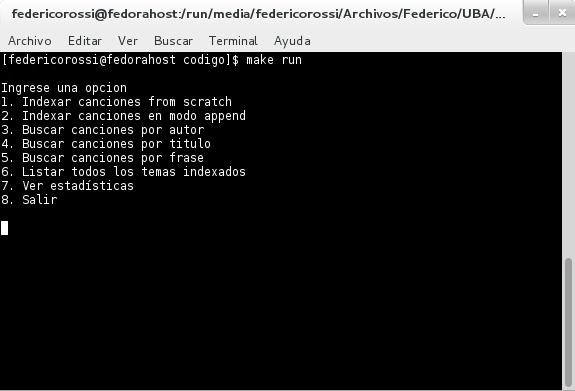
\includegraphics[width=0.85\textwidth]{images/menu.png}
	\medskip
	\caption{Menú principal del programa.}
\end{figure}
\bigskip\smallskip



% UTILIZACION DE LA INTERFAZ DEL PROGRAMA - Indexacion de canciones
\subsection{Indexación de canciones}

	Para realizar la indexación inicial de canciones debe dirigirse a la opción 1. La aplicación recorrerá el directorio de temas, generando todas las estructuras desde cero. Es necesario elegir esta opción cuando se realice la primera ejecución del programa o cuando se realicen cambios en el archivos de configuración ``\textit{parametros.conf}''.
\bigskip



% UTILIZACION DE LA INTERFAZ DEL PROGRAMA - Indexacion en modo append
\subsection{Indexación de canciones en modo append}

	Este tipo de indexación se realiza desde la opción 2 del menú. Ál elegirla, se recorrerá el directorio de temas pero sólo se indexarán los temas nuevos que aparezcan. En caso de notar problemas de performance en las búsquedas reindexar con la opción 1. No utilizar esta opción si se realizaron cambios en el archivo de configuración ``\textit{parametros.conf}''.
\bigskip



% UTILIZACION DE LA INTERFAZ DEL PROGRAMA - Busqueda de canciones por autor
\subsection{Búsqueda de canciones por autor}

	Para realizar una buesqueda de canciones indexadas por autor elija la opción 3. La búsqueda es exacta y deberá incluirse el nombre completo de la banda/autor. Se retornarán por pantalla todos los temas que coincidan con la búsqueda, y se depositarán en el archivo ``\textit{salida.out}'' las letras de dichas canciones.
\bigskip



% UTILIZACION DE LA INTERFAZ DEL PROGRAMA - Busqueda de canciones por titulo
\subsection{Búsqueda de canciones por título}

	La opción 4 del menú permite buscar canciones indexadas por título. La búsqueda es exacta y deberá incluirse el nombre completo del tema. Se retornarán por pantalla todos los temas que coincidan con la búsqueda, y se depositarán en el archivo ``\textit{salida.out}'' las letras de dichas canciones.
\bigskip



% UTILIZACION DE LA INTERFAZ DEL PROGRAMA - Busqueda de canciones por frase
\subsection{Búsqueda de canciones por frase}

	Por último, la opción 5 permite la busqueda de canciones por frase. Se retornarán por pantalla todos los temas que coincidan con la búsqueda, y se depositarán en el archivo ``\textit{salida.out}'' las letras de dichas canciones.
\bigskip\bigskip



% RESTRICCIONES
\section{Consideraciones finales}

	Para finalizar, debe tenerse en cuenta que habiéndose especificado un tamaño específico de bloque y posterior a eso se realiza una indexación, luego, las reindexaciones en modo append, así como también las búsquedas, deben realizarse manteniendo esta configuración. Es decir, si se realiza una indexación, se sale del programa, se cambia el tamaño de bloque y se vuelve a abrir, la aplicación ya no se encontrará en condiciones de utilizar correctamente lo ya indexado. Queda en la responsabilidad del usuario mantener esta limitación dada por el programa.
\bigskip


\end{document}
